\documentclass[10pt,letterpaper]{article}

\usepackage{ccn}
\usepackage{pslatex}
\usepackage{apacite}
\usepackage{graphicx}
\usepackage{caption}
\usepackage{natbib}
\usepackage{float}
\usepackage[hidelinks]{hyperref}
\usepackage{url}
\usepackage{booktabs}
\usepackage{amsfonts}
\usepackage{nicefrac}
\usepackage{microtype}
\usepackage{xcolor}
\usepackage{amsmath}
\usepackage{amssymb}
\usepackage{mathtools}
\usepackage{amsthm}
\usepackage{tabularx}
\usepackage[labelfont=bf, margin=0.8cm, font=sf]{caption}

\newcommand{\grapheme}[1]{$\langle$#1$\rangle$}

\title{Politics or Print? Separating Content from Shortcuts when Classifying\\
Two Nineteenth-Century isiXhosa Newspapers}

\author{{\large \bf Sibonelo Mlambo (536187)} \\ University of the Witwatersrand, 1 Jan Smuts Ave,\\ Braamfontein, Johannesburg, 2000, South Africa}

\begin{document}

\maketitle
\phantom{.}
\newpage
\phantom{.}
\newpage

%=====================================================================
\section{Abstract}
{\bf \looseness=-1
We ask whether a classifier that separates \emph{Imvo Zabantsundu}, founded by J.\,T.\ Jabavu in 1884, from the missionary \emph{Isigidimi sama-Xosa} reads politics or print. Using the isiXhosa Intellectual Traditions corpus (Nov 1884--1888), we train tuned classifiers along a ladder that removes English, self-references, names and spelling conventions, and add non-content baselines, matching and noise injection. Raw text is separated with balanced accuracy 0.93, but spelling and transcription features alone reach 0.85. A content-word model keeps 0.81 (0.78 on noise- and spelling-matched pairs), and its features and a lexicon show Imvo using political vocabulary at about twice Isigidimi's rate. Isigidimi's political share fell after Jabavu left, but on earlier years the classifier mainly tracks time drift.
}
\begin{quote}
\small
\textbf{Keywords:} historical isiXhosa; shortcut learning; responsible NLP
\end{quote}

%=====================================================================
\section{Introduction} \label{Intro}
\looseness=-1
\emph{Isigidimi sama-Xosa} (Lovedale, 1870--1888) was published under missionary control. \emph{Imvo Zabantsundu} (King William's Town, from November 1884) was founded by John Tengo Jabavu, who had edited Isigidimi from 1881 \citep{sahojabavu} and left because the missionaries were reluctant to publish explicitly political material \citep{odendaal1984vukani}. The digitised archive of \citet{schoots2023isixhosa} makes the split testable: if the break was political, the papers should differ in \emph{what} they discuss. A source classifier looks like natural evidence, but classifiers exploit whatever separates the labels \citep{gururangan2018annotation,geirhos2020shortcut}, and historical text is full of such shortcuts: collection-specific transcription error \citep{hill2019quantifying,vanstrien2020assessing}, mastheads, adverts and house spelling.

\textbf{Research question.} \emph{When a classifier separates the two papers over the years both appeared, how much of the separation is content, and how much is identity, transcription noise and orthography?} We test whether (H1) raw accuracy is inflated by shortcuts, (H2) a signal survives their removal, and (H3) that residual is political rather than religious. In a low-resource language \citep{joshi2020state}, mistaking print for politics would yield confident, false claims about historical Black writers.



\setlength{\belowcaptionskip}{-8pt}
\begin{figure}[t]
  \centering
  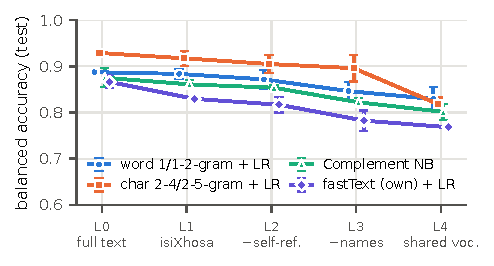
\includegraphics[width=\linewidth]{fig1_ladder_col.pdf}
  \vspace{-14pt}
  \caption{\looseness=-1 Test balanced accuracy (chance $=0.5$) as shortcuts are removed; mean $\pm$ s.d.\ over three issue-grouped splits. The character model, which can read spelling, loses most when orthography is equalised (L3$\to$L4).}
  \label{fig:ladder}
\end{figure}
\setlength{\belowcaptionskip}{0pt}

%---------------------------------------------------------------------
\begin{figure*}[t]
  \centering
  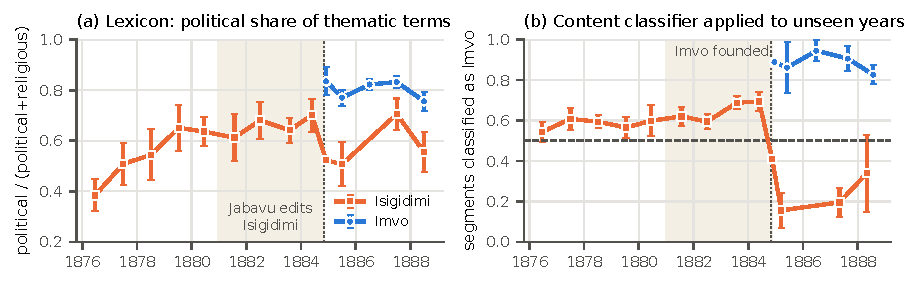
\includegraphics[width=0.9\textwidth]{fig2_eras.pdf}
  \vspace{-4pt}
  \caption{\looseness=-1 Isigidimi before, during (shaded) and after Jabavu's editorship, with Imvo for comparison; 1884 is split at Imvo's founding, and bars show $\pm1.96$ s.e.\ over issues. \textbf{(a)} Isigidimi's political share of thematic terms rises into the Jabavu years and falls after his departure. \textbf{(b)} Share of segments the L4 content model (trained on Nov 1884--88) labels ``Imvo''. Earlier years land on the Imvo side whoever the editor was, so this score tracks distance from late Isigidimi.}
  \label{fig:eras}
\end{figure*}


%=====================================================================
\section{Methods}\label{Methods}
\looseness=-1
\textbf{Data.} We use both papers from November 1884 (Imvo's first issue) to December 1888 (Isigidimi's last; its 1886 volume is lost). Pages are cut into 200-token windows (6{,}699 Imvo and 1{,}509 Isigidimi segments from 211 and 38 issues), and every cleaning level is applied to the same windows. Splits are 70/15/15 \emph{by issue}, stratified by paper and year, for three seeds. Evaluation segments sharing over 30\% of their word 6-grams with training text (reprinted adverts) are removed: 277 of 2{,}512.

\textbf{Cleaning ladder.} L0 is the full page; L1 keeps only the dataset's isiXhosa paragraphs (Imvo is 27\% English, Isigidimi 1\%; \citealp{schoots2023isixhosa}). L2 also removes self-references (titles, place of printing, staff), digits and punctuation. L3 also masks capitalised non-sentence-initial tokens (names). L4 is lower-cased, equalises orthography (\grapheme{bh}$\to$\grapheme{b}, \grapheme{xh}$\to$\grapheme{x}, no elision apostrophes) and keeps the 3{,}485 words seen $\geq5$ times in \emph{both} papers' training data, so one-paper spellings and OCR errors are unusable.

\textbf{Models.} Word and character (2--5-gram) TF-IDF with class-balanced logistic regression, Complement Naive Bayes, and fastText subword embeddings \citep{bojanowski2017enriching} trained on the training split and mean-pooled. Pretrained encoders \citep{alabi2022adapting} could not be downloaded here. Hyper-parameters are grid-searched on validation macro-F1 (scores plateau beyond the grid edge; Supp.\ Table~\ref{tab:s3}), and each test set is used once. Isigidimi is 18\% of segments, so we report macro-F1 and balanced accuracy (BA) with 95\% CIs from a bootstrap over issues.

\textbf{Isolating the signal.} (i) \emph{Feature families} on L4: the 100 most frequent shared words (a function-word ``style'' set; \citealp{mosteller1964inference}) versus the remaining ``content'' words. On raw text: 15 transcription-quality features (e.g.\ vowel-less tokens, English function words) and 4 orthographic rates (\grapheme{bh}, \grapheme{xh}, elision, hyphens). (ii) \emph{Matching}: each Isigidimi test segment is paired 1:1 with its nearest Imvo segment on the 19 standardised non-content features, within a median-distance caliper \citep{stuart2010matching}. This gives 134 pairs and cuts the mean absolute standardised difference from 0.29 to 0.08. (iii) OCR-style \emph{noise injection} (\emph{u}/\emph{n}, \emph{rn}/\emph{m}, \dots) into Isigidimi test text; (iv) a \emph{temporal hold-out} (test on 1888). (v) \emph{Probe}: the content model scores unseen Isigidimi issues from 1876--80 (before Jabavu) and 1881--Oct 1884 (under Jabavu). (vi) \emph{Lexicon}: 12 political stems (e.g.\ \emph{palamente} parliament, \emph{rulumente} government) and 12 religious stems (e.g.\ \emph{Tixo} God), with false matches removed after checking concordances (Supp.\ S2).

%---------------------------------------------------------------------
\setlength{\belowcaptionskip}{-6pt}
\begin{table}[t]
\centering
\captionsetup{font=sf, width=0.98\linewidth, skip=4pt}
\caption{\looseness=-1 Test results: macro-F1 with issue-bootstrap 95\% CI (seed 13), its s.d.\ over 3 splits, BA, and BA$_m$ on the 134 matched pairs. Majority-class macro-F1 $\approx 0.45$.}
\footnotesize
\setlength{\tabcolsep}{2.2pt}
\begin{tabular}{@{}lcccc@{}}
\toprule
Representation & Macro-F1 [CI] & s.d. & BA & BA$_m$ \\
\midrule
Full page text, char n-grams & 0.926 [0.90, 0.95] & 0.010 & 0.92 & -- \\
isiXhosa only, char n-grams & 0.916 [0.88, 0.95] & 0.012 & 0.91 & 0.86 \\
isiXhosa only, words & 0.883 [0.85, 0.92] & 0.009 & 0.88 & 0.85 \\
Shared vocab., words (uni+bi) & 0.840 [0.79, 0.88] & 0.019 & 0.84 & 0.81 \\
Shared vocab., fastText & 0.738 [0.70, 0.78] & 0.002 & 0.78 & -- \\
Content words only & 0.802 [0.76, 0.84] & -- & 0.81 & 0.78 \\
Top-100 (function) words only & 0.718 [0.68, 0.76] & -- & 0.75 & 0.71 \\
Transcription features (GB) & 0.715 [0.66, 0.77] & -- & 0.74 & 0.62 \\
Orthography features (GB) & 0.759 [0.69, 0.82] & -- & 0.83 & 0.73 \\
All non-content features (GB) & 0.831 [0.78, 0.87] & -- & 0.85 & 0.75 \\
\bottomrule
\end{tabular}
\label{tab:main}
\end{table}
\setlength{\belowcaptionskip}{0pt}

%=====================================================================
\section{Results}\label{Results}
\looseness=-1
\textbf{Shortcuts inflate accuracy (H1).} On full pages character $n$-grams reach BA $0.93\pm0.01$ (Fig.~\ref{fig:ladder}). The strongest L1 character features are house conventions: Imvo writes \grapheme{bh} (8.7 tokens per 1{,}000 vs.\ 0.01) and \grapheme{xh}, while Isigidimi uses elision apostrophes three times as often. Imvo also has 2.4$\times$ more vowel-less tokens, mostly residual transcription errors. Non-content features alone reach BA 0.85 (Table~\ref{tab:main}). Disabling the reprint filter changes scores by $<0.01$.

\textbf{A content signal survives (H2).} Each control lowers accuracy, but the L4 word model keeps BA $0.83\pm0.03$ across splits, and content words alone reach 0.81. On matched pairs the content model loses only 0.03, while the non-content models lose 0.10--0.12 (Table~\ref{tab:main}, BA$_m$). Matching is imperfect, so this bounds the confound. Corrupting 5\% of Isigidimi tokens moves under 4\% of segments to ``Imvo''. Tested on unseen 1888, the L4 model keeps BA 0.80. Our own fastText embeddings (about 1M training tokens) trail sparse features throughout.

\textbf{The residual is political (H3).} Top Imvo content features include \emph{abamnyama} and \emph{amawetu} (``black people'', ``our people''), \emph{imantyi} (magistrate), \emph{amatyala} (court cases), \emph{entolongweni} (in prison) and Gordon Sprigg, Cape premier from 1886. Isigidimi's include \emph{imbali} (history), \emph{inkosi} (chief), \emph{imfazwe} (war) and \emph{Ntsikana}, the early Xhosa Christian hymn-writer. Imvo uses 14.1 political terms per 1{,}000 tokens [13.3, 14.8] against Isigidimi's 7.4 [6.2, 8.7] (permutation $p<0.001$), and 3.2 vs.\ 5.1 religious terms. Within Isigidimi (Fig.~\ref{fig:eras}a), the political share rises from 0.54 [0.49, 0.58] in 1876--80 to 0.67 [0.63, 0.70] under Jabavu, then falls to 0.59 [0.54, 0.63] after he left.

\textbf{The classifier is a poor clock.} On unseen Isigidimi years (Fig.~\ref{fig:eras}b) the content model calls 66\% of Jabavu-era segments ``Imvo'', but also 58\% of 1876--80 segments, against 26\% of held-out post-1884 ones. The Jabavu-era excess over 1876--80 is small (+0.05 mean probability, CI [0.03, 0.07]). It learned ``unlike late Isigidimi'', not ``like Imvo''.


%=====================================================================
\section{Discussion}\label{Discussion}
\looseness=-1
Print alone separates the papers (BA 0.85 without a topic word), so a 0.93 source classifier is no evidence of a political split (H1). Only after the controls does accuracy become interpretable, and it stays near 0.8 because the content differs (H2). Imvo's distinctive vocabulary is political, Isigidimi's historical and Christian (H3). This fits the account that Jabavu left to write politics freely \citep{odendaal1984vukani}: Isigidimi's political share peaked in his last years there and then fell. Its rise began in the late 1870s, however, suggesting a gradual politicisation that Isigidimi did not sustain rather than a single editor effect. We do not judge whether Jabavu was ``right'' to leave.

\textbf{Responsible NLP.} \emph{Ablate before interpreting:} L1 feature weights would have presented \grapheme{bh} and apostrophes as Imvo's ``voice''. \emph{Noise is partly culture:} Imvo's spelling (e.g.\ \emph{Xhosa}, never printed in Isigidimi) is plausibly an editorial choice; removing it suits questions of topic, not identity, and must be documented \citep{bender2018data}. \emph{Forced-choice models misread time:} a binary classifier puts every unfamiliar text into one of its two classes, so Fig.~\ref{fig:eras}b does not show that 1876 Isigidimi ``sounded like'' Imvo. Such outputs must not become ideological labels for named authors \citep{blodgett2020language}.

\textbf{Limitations.} Isigidimi supplies 38 issues (about 7 per test split), so CIs are wide. The lexicons, built by a non-first-language speaker, impose a modern politics/religion split on writers for whom the two were entwined. Publication frequency and genre are confounded with source, and word division survives L4 (Imvo's separated prefixes \emph{base}, \emph{ase} rank highly). 

%=====================================================================
\section{Contribution Statement}
This was an individual project; the author list is unchanged from the preliminary statement. Sibonelo Mlambo is responsible for all components: reading the background literature, data exploration, experiment design (hypotheses, controls, splits and metrics), implementation of the pipeline and models, analysis, and writing of this abstract, the ethics checklist and the code documentation. Compared with the preliminary statement, (i) the pretrained multilingual model was replaced by fastText embeddings trained on the corpus, because pretrained weights could not be downloaded in the compute environment; (ii) topic modelling was replaced by feature-family ablations and a validated thematic lexicon, which answered the question more directly; and (iii) non-content matching, noise injection, a temporal hold-out and an out-of-sample probe of earlier Isigidimi years were added. AI assistance was used as declared below.

\section{Faculty of Science AI Ethics Statement}
I declare that generative AI was used in this project, as permitted by the course brief. Claude (Anthropic), used through an agentic coding environment, assisted with: designing the experimental controls, writing and debugging the Python code in the submission, running the experiments, producing the figures, and drafting the text of this extended abstract, the README and the NeurIPS checklist answers. Every claim and number in the abstract was checked against the experiment outputs (\texttt{outputs/results.csv}, \texttt{outputs/stats.json}), and historical facts were checked against the cited sources. The isiXhosa glosses are limited to words whose meaning I could verify, and the thematic lexicons were checked against corpus concordances. I have read and understood all code and text in this submission and take full responsibility for it, including any errors. No AI system was used to generate data or annotations for the experiments.

\bibliographystyle{apacite}
\setlength{\bibleftmargin}{.125in}
\setlength{\bibindent}{-\bibleftmargin}
\bibliography{refs}

\clearpage
\onecolumn
% NeurIPS 2024 Paper Checklist (questions reproduced from the NeurIPS 2024 template).
% If the course-provided .tex differs in wording, paste these answers into it.
\newcommand{\answerYes}[1][]{\textcolor{blue}{[Yes] #1}}
\newcommand{\answerNo}[1][]{\textcolor{orange}{[No] #1}}
\newcommand{\answerNA}[1][]{\textcolor{gray}{[NA] #1}}

\section*{NeurIPS Paper Checklist}
\begin{enumerate}

\item {\bf Claims}
    \item[] Question: Do the main claims made in the abstract and introduction accurately reflect the paper's contributions and scope?
    \item[] Answer: \answerYes{}
    \item[] Justification: The abstract and introduction claim that (i) raw-text source classification is inflated by non-content shortcuts (spelling and transcription proxies alone reach balanced accuracy 0.85), (ii) a source signal survives all controls (about 0.8), which the paper explicitly does not attribute exclusively to politics, and (iii) a separate lexicon analysis shows more political vocabulary in Imvo, including within every common year. Each claim is tied to Table 1, a figure or a supplementary table. The scope is two newspapers from November 1884 to December 1888, plus earlier Isigidimi issues used only as a probe.

\item {\bf Limitations}
    \item[] Question: Does the paper discuss the limitations of the work performed by the authors?
    \item[] Answer: \answerYes{}
    \item[] Justification: The Limitations paragraph, Methods and Supplement note the small number of Isigidimi issues (38; wide confidence intervals), the missing 1886 Isigidimi volume, the hand-built lexicons (drafted by a non-first-language speaker, not reviewed by a first-language speaker, without estimated precision, with several patterns that also carry non-political or non-religious senses, and imposing a modern politics/religion split), the confounding of publication frequency and genre with source, the loose separation of style and topic by word frequency, matching that reduces only measured imbalance, transcription features that are proxies rather than measured OCR error rates, and the absence of pretrained encoders. The Discussion explains why the out-of-sample classifier probe cannot be read as an editor effect, and the follow-up analyses added after inspecting results are labelled exploratory.

\item {\bf Theory Assumptions and Proofs}
    \item[] Question: For each theoretical result, does the paper provide the full set of assumptions and a complete (and correct) proof?
    \item[] Answer: \answerNA{}
    \item[] Justification: The paper is empirical and contains no theoretical results.

\item {\bf Experimental Result Reproducibility}
    \item[] Question: Does the paper fully disclose all the information needed to reproduce the main experimental results of the paper to the extent that it affects the main claims and/or conclusions of the paper (regardless of whether the code and data are provided or not)?
    \item[] Answer: \answerYes{}
    \item[] Justification: The Methods section and Supplement specify the segmentation (200-token windows), the cleaning ladder L0--L4, the issue-grouped 70/15/15 split stratified by paper and year, the near-duplicate filter, the model families and hyper-parameter grids (Supplement S1), the matching procedure and the noise-injection procedure. Random seeds are fixed in the code; fastText is trained single-threaded with a fixed \texttt{PYTHONHASHSEED}, so reruns with the pinned package versions are deterministic.

\item {\bf Open access to data and code}
    \item[] Question: Does the paper provide open access to the data and code, with sufficient instructions to faithfully reproduce the main experimental results, as described in supplemental material?
    \item[] Answer: \answerYes{}
    \item[] Justification: The code, a \texttt{requirements.txt} with pinned versions, a \texttt{README.txt}, a one-command script (\texttt{reproduction.sh}) and a Colab notebook are publicly available at \url{https://github.com/SiboneloMlambo/NLP_COMS7066A} (folder \texttt{Project2\_isiXhosa}). The newspaper text itself is not redistributed there (see the licence answer below); the README explains how to obtain and place it.

\item {\bf Experimental Setting/Details}
    \item[] Question: Does the paper specify all the training and test details (e.g., data splits, hyperparameters, how they were chosen, type of optimizer, etc.) necessary to understand the results?
    \item[] Answer: \answerYes{}
    \item[] Justification: The splits, grids and selection criterion (validation macro-F1, test set used once) are described in Methods; the selected hyper-parameters for every run are written to \texttt{outputs/results.csv}.

\item {\bf Experiment Statistical Significance}
    \item[] Question: Does the paper report error bars suitably and correctly defined or other appropriate information about the statistical significance of the experiments?
    \item[] Answer: \answerYes{}
    \item[] Justification: Test scores carry 95\% confidence intervals from a cluster bootstrap that resamples whole issues (1{,}000 resamples); for the matched subset, the matched segments are held fixed and issues are resampled within each newspaper. The standard deviation over three independent issue splits is also reported. Lexicon differences use issue-level bootstrap intervals and permutation tests (within year for the year-controlled comparison).

\item {\bf Experiments Compute Resources}
    \item[] Question: For each experiment, does the paper provide sufficient information on the computer resources (type of compute workers, memory, time of execution) needed to reproduce the experiments?
    \item[] Answer: \answerYes{}
    \item[] Justification: All experiments run on CPU only (2 virtual cores, 8\,GB RAM, no GPU). The full pipeline (three seeds, all models including single-threaded fastText, plus the grid-edge check) takes about 75 minutes of wall-clock time with \texttt{reproduction.sh}, which runs the seeds in two parallel processes; \texttt{--fast} skips fastText.

\item {\bf Code Of Ethics}
    \item[] Question: Does the research conducted in the paper conform, in every respect, with the NeurIPS Code of Ethics \url{https://neurips.cc/public/EthicsGuidelines}?
    \item[] Answer: \answerYes{}
    \item[] Justification: The work uses publicly archived historical newspapers (1884--1888), involves no living human subjects, releases no generative model, and discusses the risks of attributing ideology to historical African authors from noisy text.

\item {\bf Broader Impacts}
    \item[] Question: Does the paper discuss both potential positive societal impacts and negative societal impacts of the work performed?
    \item[] Answer: \answerYes{}
    \item[] Justification: Positive: the work gives digital humanities researchers a concrete control protocol before drawing cultural conclusions from OCR-derived isiXhosa archives. Negative: source and stance classifiers trained on such data can turn digitisation artefacts and modern categories into confident but wrong claims about historical Black South African writers and their politics, and can misattribute anonymous or pseudonymous writing; the Discussion addresses this.

\item {\bf Safeguards}
    \item[] Question: Does the paper describe safeguards that have been put in place for responsible release of data or models that have a high risk for misuse (e.g., pretrained language models, image generators, or scraped datasets)?
    \item[] Answer: \answerNA{}
    \item[] Justification: No new dataset or high-risk model is released; the classifiers are small linear models trained for analysis only.

\item {\bf Licenses for existing assets}
    \item[] Question: Are the creators or original owners of assets (e.g., code, data, models), used in the paper, properly credited and are the license and terms of use explicitly mentioned and properly respected?
    \item[] Answer: \answerYes{}
    \item[] Justification: The texts come from the isiXhosa Intellectual Traditions Digital Archive (Department of Sociology, University of Cape Town; \citealp{schoots2023isixhosa}). The archive's item pages state that the Word documents are ``downloadable and reusable'' without naming a licence, while UCT's eMandulo/Five Hundred Year Archive mirror of the converted text files marks them CC BY-NC-ND 4.0. We therefore use them only for non-commercial coursework, credit the source, and do not redistribute the text or derived corpora in our public repository. High-resolution scans belong to the National Library of South Africa and were not used. Software (scikit-learn, gensim, NumPy, pandas, SciPy, Matplotlib) is open source and listed with versions in \texttt{requirements.txt}.

\item {\bf New Assets}
    \item[] Question: Are new assets introduced in the paper well documented and is the documentation provided alongside the assets?
    \item[] Answer: \answerYes{}
    \item[] Justification: The only new assets are the analysis code and two small thematic lexicons (in \texttt{src/features.py}), documented in the README and in code comments with the gloss of every stem.

\item {\bf Crowdsourcing and Research with Human Subjects}
    \item[] Question: For crowdsourcing experiments and research with human subjects, does the paper include the full text of instructions given to participants and screenshots, if applicable, as well as details about compensation (if any)?
    \item[] Answer: \answerNA{}
    \item[] Justification: No crowdsourcing or human-subject research was performed.

\item {\bf Institutional Review Board (IRB) Approvals or Equivalent for Research with Human Subjects}
    \item[] Question: Does the paper describe potential risks incurred by study participants, whether such risks were disclosed to the subjects, and whether Institutional Review Board (IRB) approvals (or an equivalent approval/review based on the requirements of your country or institution) were obtained?
    \item[] Answer: \answerNA{}
    \item[] Justification: No human participants were involved.

\end{enumerate}


\clearpage
\twocolumn
\section*{Supplementary Material}
\textbf{S1. Implementation details.} Segments are 200 whitespace tokens (windows with fewer than 60 raw or 30 L4 tokens are dropped). Grids: word LR $C\in\{0.3,1,3,10,30\}$, $n$-grams $\{(1,1),(1,2)\}$, min.\ df $\{2,5\}$; char LR $C\in\{1,3,10,30\}$, $n\in\{(2,4),(2,5)\}$; Complement NB $\alpha\in\{0.01,0.03,0.1,0.3,1\}$, min.\ df $\{2,5\}$; fastText (skip-gram, window 5, subwords 3--5, 10 epochs, 200k hash buckets) dim $\{50,100\}$ with LR $C\in\{0.01,0.1,1\}$; non-content LR $C\in\{10^{-3},\dots,10^{2}\}$; histogram gradient boosting learning rate $\{0.05,0.1\}$, depth $\{2,3,5\}$. All logistic regressions are class-balanced. Selected values for every run are in \texttt{outputs/results.csv}. Software: scikit-learn \citep{pedregosa2011scikit}, gensim \citep{rehurek2010software}. Compute: CPU only (2 cores, 8\,GB RAM); about 65 minutes wall-clock with the two README commands run in parallel.

\textbf{S2. Lexicons} (stems matched inside lower-cased tokens; old orthography). \emph{Political:} palamente (parliament), voti/vota (vote), nyulo/nyulw/nyula (elect, election; excluding \emph{-qanyul-} ``cut''), rulumen (government), mteto/miteto (law), lungelo (right), rafu (tax), mantyi (magistrate), tyala (court case, charge), koloni (the Colony), bhunga (council). \emph{Religious:} tixo (God), yesu (whole word), kristu (Christ), tandaz (pray), zibalo (scripture), vangeli (gospel), ngcwele (holy), sono (sin, word-final), mfundisi/bafundisi (minister/s), cawa (church, Sunday), nkonzo (service). Rejected after concordance checks: \emph{kolwa} (matches \emph{kolwandle}), \emph{bunga} (many unrelated words), \emph{lawul} (mostly \emph{hlawula}, ``pay'').

\textbf{S3. Synthetic noise.} The noisier paper was identified by its rate of vowel-less plus mixed letter--digit tokens (Imvo 3.8\% vs.\ Isigidimi 1.4\% of tokens; rare-token rate was not used because it is confounded with each paper's share of the training vocabulary). Confusions were injected into Isigidimi test segments at 0--40\% of tokens (Fig.~\ref{fig:s1}).

\begin{figure*}[h]
\centering
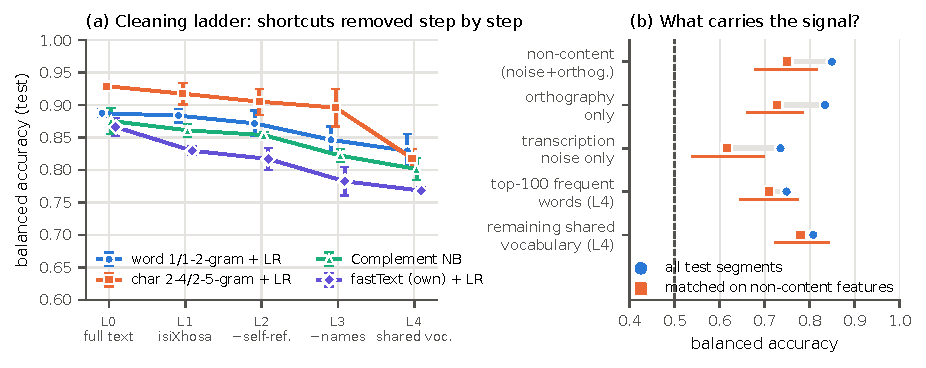
\includegraphics[width=\textwidth]{fig1_ladder.pdf}
\caption{Extended version of Fig.~\ref{fig:ladder}. \textbf{(b)} Single feature families (seed 13) on all test segments (blue) and on the 134 pairs matched for the 19 non-content features (orange): matching costs the content model 0.03 but the non-content models 0.10--0.12.}
\label{fig:s0}
\end{figure*}

\begin{figure}[h]
\centering
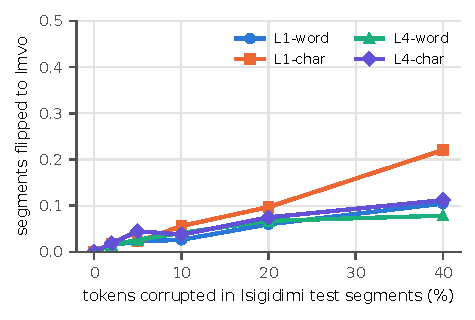
\includegraphics[width=\linewidth]{figS1_noise.pdf}
\caption{Share of Isigidimi test segments classified as Imvo as synthetic OCR confusions are injected. Realistic rates (2--5\%) barely move predictions; only implausibly heavy corruption shifts the raw character model.}
\label{fig:s1}
\end{figure}

\begin{figure*}[h]
\centering
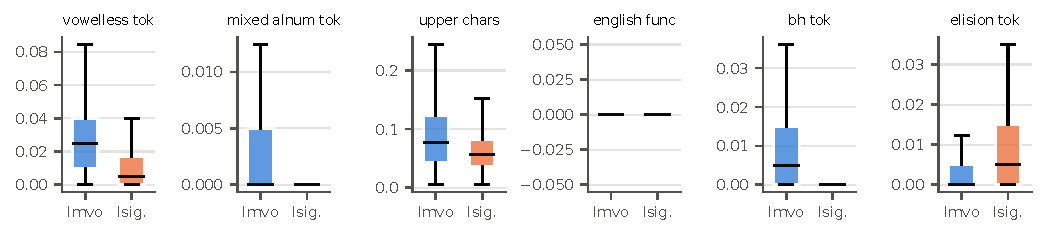
\includegraphics[width=\textwidth]{figS2_surface.pdf}
\caption{Selected non-content features per segment (training split; boxes: interquartile range, whiskers: 1.5 IQR). Imvo has more vowel-less and mixed letter--digit tokens, uppercase characters and English function words; the \grapheme{bh} digraph is almost exclusive to Imvo and apostrophe elision is more frequent in Isigidimi.}
\label{fig:s2}
\end{figure*}

\begin{table}[h]\centering\small\caption{Cleaning ladder, test macro-F1 / balanced accuracy, mean $\pm$ s.d.\ over three issue-grouped splits (seeds 13, 21, 42).}
\begin{tabular}{@{}llcc@{}}\toprule Level & Model & Macro-F1 & Bal.\ acc. \\ \midrule
L0 & char & 0.937 $\pm$ 0.010 & 0.929 $\pm$ 0.007 \\
L0 & fastText & 0.829 $\pm$ 0.028 & 0.866 $\pm$ 0.014 \\
L0 & CNB & 0.812 $\pm$ 0.029 & 0.875 $\pm$ 0.020 \\
L0 & word & 0.902 $\pm$ 0.008 & 0.887 $\pm$ 0.006 \\
L1 & char & 0.927 $\pm$ 0.012 & 0.917 $\pm$ 0.017 \\
L1 & fastText & 0.807 $\pm$ 0.015 & 0.830 $\pm$ 0.007 \\
L1 & CNB & 0.857 $\pm$ 0.021 & 0.861 $\pm$ 0.010 \\
L1 & word & 0.891 $\pm$ 0.009 & 0.884 $\pm$ 0.011 \\
L2 & char & 0.916 $\pm$ 0.017 & 0.905 $\pm$ 0.020 \\
L2 & fastText & 0.798 $\pm$ 0.014 & 0.817 $\pm$ 0.017 \\
L2 & CNB & 0.852 $\pm$ 0.016 & 0.854 $\pm$ 0.005 \\
L2 & word & 0.886 $\pm$ 0.013 & 0.872 $\pm$ 0.020 \\
L3 & char & 0.906 $\pm$ 0.025 & 0.896 $\pm$ 0.029 \\
L3 & fastText & 0.758 $\pm$ 0.025 & 0.783 $\pm$ 0.022 \\
L3 & CNB & 0.819 $\pm$ 0.013 & 0.822 $\pm$ 0.010 \\
L3 & word & 0.859 $\pm$ 0.016 & 0.846 $\pm$ 0.020 \\
L4 & char & 0.816 $\pm$ 0.007 & 0.818 $\pm$ 0.015 \\
L4 & fastText & 0.737 $\pm$ 0.018 & 0.768 $\pm$ 0.005 \\
L4 & CNB & 0.767 $\pm$ 0.009 & 0.801 $\pm$ 0.017 \\
L4 & word & 0.839 $\pm$ 0.019 & 0.829 $\pm$ 0.026 \\
\bottomrule\end{tabular}\label{tab:s1}\end{table}
\begin{table}[h]\centering\small\caption{Robustness (seed 13). \emph{No dedup}: near-duplicate filter switched off. \emph{Temporal}: train/validate on Nov 1884--1887, test on 1888. Reference: the main random split.}
\begin{tabular}{@{}lllcc@{}}\toprule Run & Level & Model & Macro-F1 & Ref.\ macro-F1 \\ \midrule
No dedup & L0 & word & 0.902 & 0.899 \\
No dedup & L0 & char & 0.928 & 0.926 \\
No dedup & L1 & word & 0.890 & 0.883 \\
No dedup & L1 & char & 0.920 & 0.916 \\
Temporal & L1 & word & 0.864 & 0.883 \\
Temporal & L1 & char & 0.896 & 0.916 \\
Temporal & L4 & word & 0.787 & 0.840 \\
Temporal & L4 & char & 0.745 & 0.811 \\
\bottomrule\end{tabular}\label{tab:s2}\end{table}
\begin{table}[h]\centering\small\caption{Grid-edge check (validation macro-F1, seed 13). Several selected $C$ values sat at the top of the grid; larger values do not improve validation scores.}
\begin{tabular}{@{}llcccc@{}}\toprule Level & Model & $C$=10 & 30 & 100 & 300 \\ \midrule
L1 & char & 0.944 & 0.948 & 0.946 & 0.946 \\
L1 & word & 0.885 & 0.888 & 0.890 & 0.886 \\
L4 & char & 0.824 & 0.813 & 0.798 & 0.795 \\
L4 & word & 0.836 & 0.824 & 0.817 & 0.815 \\
\bottomrule\end{tabular}\label{tab:s3}\end{table}
\begin{table*}[h]\centering\small\caption{Editorial eras. Lexicon rates per 1{,}000 tokens (issue-level means, bootstrap 95\% CI over issues; all issues). Probe: mean P(Imvo) from the L4 content model and share of segments classified Imvo (post-1884 rows: held-out test issues only).}
\begin{tabular}{@{}lcccccc@{}}\toprule Group & Issues (lex.) & Political/1k & Religious/1k & Political share & Mean P(Imvo) & \% segs.\ Imvo \\ \midrule
Isigidimi 1876-80 (pre-Jabavu) & 51 & 8.93 [8.12, 9.80] & 8.23 [7.08, 9.40] & 0.54 [0.49, 0.58] & 0.55 & 58 \\
Isigidimi 1881-Oct 1884 (Jabavu) & 56 & 10.04 [9.00, 11.12] & 4.76 [4.22, 5.34] & 0.67 [0.63, 0.70] & 0.60 & 66 \\
Isigidimi Nov 1884-88 (post-Jabavu) & 38 & 7.38 [6.22, 8.73] & 5.14 [4.32, 5.98] & 0.59 [0.54, 0.63] & 0.34 & 26 \\
Imvo Nov 1884-88 & 211 & 13.97 [13.24, 14.70] & 3.23 [3.01, 3.47] & 0.80 [0.78, 0.81] & 0.78 & 88 \\
\bottomrule\end{tabular}\label{tab:s4}\end{table*}
\begin{table}[h]\centering\small\caption{Twenty largest-weight features of the L4 content model, in order (seed 13). Glosses for selected items are given in the Results.}
\begin{tabular}{@{}p{0.45\linewidth}p{0.45\linewidth}@{}}\toprule Favour Imvo & Favour Isigidimi \\ \midrule
\emph{njengokuba, abamnyama, mayelana, base, ase, uku, sprigg, egqitileyo, kukuba, ba, zetu, epepeni, suka, omnyama, ixabiso, oka, okokuba, lokuba, amawetu, kwelilizwe} & \emph{imbali, ed, ngoko, ngosuku, malunga, uzele, suke, ezinje, londawo, inani, um, kanjalo, mbali, evekini, umlambo, ngolwe, ingu, ngxoxo, kwase, ndawo} \\
\bottomrule\end{tabular}\label{tab:s5}\end{table}
\begin{table}[h]\centering\small\caption{Matched evaluation (seed 13): balanced accuracy on all test segments and on the matched pairs, with a 95\% CI from resampling pairs (1{,}000 resamples).}
\begin{tabular}{@{}lccc@{}}\toprule Model & BA (all) & BA (matched) & 95\% CI \\ \midrule
L1 words & 0.880 & 0.854 & [0.81, 0.90] \\
L1 char & 0.906 & 0.862 & [0.82, 0.90] \\
L2 words & 0.857 & 0.832 & [0.79, 0.87] \\
L2 char & 0.897 & 0.851 & [0.81, 0.89] \\
L3 words & 0.847 & 0.802 & [0.76, 0.84] \\
L3 char & 0.880 & 0.832 & [0.79, 0.87] \\
L4 words & 0.837 & 0.810 & [0.76, 0.85] \\
L4 char & 0.814 & 0.806 & [0.76, 0.85] \\
Transcription (LR) & 0.687 & 0.578 & [0.54, 0.61] \\
Transcription (GB) & 0.735 & 0.616 & [0.57, 0.66] \\
Orthography (LR) & 0.831 & 0.735 & [0.69, 0.78] \\
Orthography (GB) & 0.834 & 0.728 & [0.68, 0.77] \\
All non-content (LR) & 0.858 & 0.750 & [0.71, 0.79] \\
All non-content (GB) & 0.849 & 0.750 & [0.70, 0.79] \\
L4 remaining vocabulary & 0.808 & 0.780 & [0.73, 0.82] \\
L4 top-100 frequent words & 0.749 & 0.709 & [0.66, 0.76] \\
L4 remaining, minus fragments/names & 0.779 & 0.746 & [0.69, 0.80] \\
\bottomrule\end{tabular}\label{tab:matched}\end{table}
\begin{table}[h]\centering\small\caption{Per-feature balance before and after matching: difference in means (Imvo $-$ Isigidimi) in training-standard-deviation units. 134 pairs from 35 issues; mean $|$SMD$|$ 0.29 $\to$ 0.08; 1 feature(s) still exceed 0.25 after matching.}
\begin{tabular}{@{}lrr@{}}\toprule Feature & Before & After \\ \midrule
mean\_tok\_len & +0.05 & +0.13 \\
sd\_tok\_len & +0.50 & +0.18 \\
short\_tok & +0.30 & +0.07 \\
long\_tok & +0.20 & +0.03 \\
upper\_chars & +0.10 & -0.11 \\
punct\_chars & -0.38 & -0.10 \\
digit\_chars & +0.08 & -0.04 \\
nonascii\_chars & +0.27 & +0.04 \\
vowelless\_tok & +0.28 & +0.08 \\
mixed\_alnum\_tok & +0.08 & -0.01 \\
rare\_tok & -0.40 & -0.08 \\
type\_token\_ratio & -0.16 & -0.02 \\
english\_func & +0.27 & -0.02 \\
cap\_initial\_tok & +0.24 & +0.03 \\
split\_fragment & -0.01 & +0.00 \\
bh\_tok & +0.82 & +0.29 \\
xh\_tok & +0.54 & +0.04 \\
elision\_tok & -0.71 & -0.22 \\
hyphen\_tok & -0.10 & -0.09 \\
\bottomrule\end{tabular}\label{tab:balance}\end{table}
\begin{table*}[h]\centering\small\caption{Year-controlled lexicon comparison: years in which both papers appear (Isigidimi 1886 is missing; 1884 = Nov--Dec). Issue-level means; CI of the difference from bootstrapping issues within the year. Political / 1k: mean within-year difference +5.91, within-year permutation $p=0.0002$; Religious / 1k: mean within-year difference -2.25, within-year permutation $p=0.0002$; Political share: mean within-year difference +0.23, within-year permutation $p=0.0002$.}
\begin{tabular}{@{}llcccccc@{}}\toprule Measure & Year & Imvo & Isigidimi & Difference & 95\% CI & Issues (I/Is) \\ \midrule
Political / 1k & 1884 & 10.85 & 6.55 & +4.30 & [1.41, 6.97] & 9/2 \\
Political / 1k & 1885 & 11.88 & 5.74 & +6.14 & [4.13, 7.90] & 49/12 \\
Political / 1k & 1887 & 15.84 & 8.75 & +7.10 & [4.11, 9.70] & 49/12 \\
Political / 1k & 1888 & 13.88 & 7.78 & +6.10 & [2.83, 9.08] & 52/12 \\
Religious / 1k & 1884 & 1.90 & 5.94 & -4.04 & [-5.36, -2.73] & 9/2 \\
Religious / 1k & 1885 & 3.32 & 5.51 & -2.19 & [-3.46, -0.86] & 49/12 \\
Religious / 1k & 1887 & 3.02 & 3.59 & -0.57 & [-1.73, 0.53] & 49/12 \\
Religious / 1k & 1888 & 3.97 & 6.19 & -2.21 & [-4.06, -0.43] & 52/12 \\
Political share & 1884 & 0.83 & 0.52 & +0.31 & [0.26, 0.36] & 9/2 \\
Political share & 1885 & 0.77 & 0.51 & +0.26 & [0.17, 0.35] & 49/12 \\
Political share & 1887 & 0.83 & 0.71 & +0.13 & [0.06, 0.19] & 49/12 \\
Political share & 1888 & 0.76 & 0.56 & +0.20 & [0.11, 0.29] & 52/12 \\
\bottomrule\end{tabular}\label{tab:yearlex}\end{table*}
\begin{table*}[h]\centering\scriptsize\caption{Lexicon audit (main window). For each pattern: matches in each paper, the five most frequent matched word types, and one randomly drawn concordance line (lower-cased, punctuation removed). Patterns were drafted from general knowledge of isiXhosa before any per-paper comparison; the concordance check removed false matches (Table~\ref{tab:rejected}) and no pattern was added or removed because of the direction of a difference. Glosses are the author's; a first-language speaker has not reviewed them.}
\begin{tabular}{@{}llrrp{0.30\textwidth}p{0.33\textwidth}@{}}\toprule Cat. & Pattern & Imvo & Isig. & Top matched types & Example context \\ \midrule
pol. & \texttt{koloni} & 1117 & 159 & \emph{koloni (1108); ikoloni (89); yasekoloni (22); mkoloni (14); umkoloni (9)} & \emph{lase bechuanaland liya kuhlonyelwa kule koloni nokuba u montsiwa seleteta ntonina} \\
pol. & \texttt{lungelo} & 1139 & 212 & \emph{amalungelo (346); ilungelo (294); lungelo (94); nelungelo (56); namalungelo (51)} & \emph{ngamatanda mfazwe encediswa zizihlobo mpi namalungelo abo ilungelo la mampondo ubelenze} \\
pol. & \texttt{mantyi} & 1847 & 155 & \emph{mantyi (605); imantyi (487); yimantyi (128); umantyi (126); yemantyi (94)} & \emph{emva kokutabata inteto yetu engokuba imantyi iyakuhlala esihlalweni ngomso edikeni ukuva} \\
pol. & \texttt{miteto} & 487 & 65 & \emph{imiteto (245); miteto (96); lemiteto (34); nemiteto (28); ngemiteto (22)} & \emph{imimiselo nemi gqaliselo nokuba yi miteto nokuba zinxalenye zayo ecaseneyo mhlaimbi} \\
pol. & \texttt{mteto} & 2206 & 278 & \emph{umteto (727); lomteto (490); mteto (368); ngomteto (173); ngumteto (99)} & \emph{nokupendula imicimbi yombuso banayo imfanelo ngomteto wokunyula owebala labo eze kulenkundla} \\
pol. & \texttt{nyula} & 324 & 41 & \emph{lokunyula (65); ukunyula (39); onganyula (24); yokunyula (16); ngokunyula (13)} & \emph{bacelwe ukuba banganqopisani namntu ungoyena bayakumnyula ade onke amadoda ayakuma abe} \\
pol. & \texttt{nyulo} & 232 & 32 & \emph{unyulo (73); wonyulo (28); lonyulo (18); yonyulo (18); nyulo (17)} & \emph{eziyakuze zibakanyele i feltkornet ngomhla wonyulo kuba zoti zakuba zibuze igama} \\
pol. & \texttt{nyulw} & 548 & 68 & \emph{kunyulwe (89); enyulwe (64); kunyulwa (45); ukunyulwa (32); anyulwe (30)} & \emph{u faku col griffith yena anyulwe eko lomadinga anjalo esenziwa ngawayesilwa} \\
pol. & \texttt{palamente} & 1842 & 114 & \emph{palamente (1857); ipalamente (46); palamenteni (31); epalamente (15); bapalamente (1)} & \emph{kokuba ade abe uyalelwe yi palamente u mr j umnumzetu unga} \\
pol. & \texttt{rafu} & 874 & 84 & \emph{irafu (400); rafu (347); lerafu (39); yerafu (35); lorafu (23)} & \emph{read lokuba bazihlaule ngexesha i rafu zabo kuba kungenakubako lulaulo ngapandle} \\
pol. & \texttt{rulumen} & 3124 & 318 & \emph{rulumente (1996); rulumeni (1410); rulumenteni (7); urulumente (5); urulumeni (3)} & \emph{gaso ' akasoia aye ku rulumeni ' makabe u qipu yinkosi} \\
pol. & \texttt{tyala} & 2349 & 300 & \emph{ityala (476); amatyala (449); tyala (247); yamatyala (138); ngetyala (66)} & \emph{laya ixelwe ekuqaleni ngokubheki selele kumatyala okwapula iziqendwana ezi zinga a} \\
pol. & \texttt{vota} & 202 & 32 & \emph{lokuvota (54); kuvota (19); ukuvota (18); vota (15); yokuvota (14)} & \emph{abantsundu ngabenga nikwanga nelungelo loku vota ayitandi inxenye yakubona sivota ke} \\
pol. & \texttt{voti} & 1051 & 175 & \emph{ivoti (299); voti (207); evotini (140); abavoti (99); ngevoti (56)} & \emph{lonto kuti amawetu anevoti makangake anikele indlebe zawo konomgogwana} \\
rel. & \texttt{\^{}yesu\$} & 30 & 48 & \emph{yesu (78)} & \emph{ibuhlungu kuba ndilele apa no yesu inkosi yam ute xa bekusondela} \\
rel. & \texttt{bafundisi} & 952 & 281 & \emph{abafundisi (436); yabafundisi (137); ngabafundisi (97); bafundisi (81); nabafundisi (77)} & \emph{ke ndiveleni obubunzima zinkosi zam bafundisi base wesileni ndiyanitandaza ndiyazitoba ndisisicaka} \\
rel. & \texttt{cawa} & 674 & 92 & \emph{cawa (478); ingcawa (156); ngcawa (64); yencawa (12); ngecawa (7)} & \emph{ibokwe inani lotnkosi ngomhla we cawa dec wawumayelana senza ityalike enkulu} \\
rel. & \texttt{kristu} & 80 & 151 & \emph{kristu (206); makristu (8); kristukazi (8); mkristu (3); amakristu (2)} & \emph{siyibona ukwapulwa kwayo lemimiselo ka kristu kwi eamente} \\
rel. & \texttt{mfundisi} & 932 & 231 & \emph{umfundisi (488); mfundisi (162); ngumfundisi (108); nomfundisi (55); yomfundisi (48)} & \emph{nokuba ngabapina ngapandle kwamatanda into egumfundisi omkulu ngezimini endaba besingati simi} \\
rel. & \texttt{ngcwele} & 75 & 42 & \emph{oyingcwele (29); ongcwele (17); ezingcwele (16); ngcwele (8); ngcweleshe (6)} & \emph{ngokufunda amaculo la ati yerusalem engcwele eyase zulwini ndilundwendwe ndingumhambi ezulwini} \\
rel. & \texttt{nkonzo} & 107 & 27 & \emph{inkonzo (85); nkonzo (8); lenkonzo (6); kwinkonzo (5); kwenkonzo (4)} & \emph{zatakazelwa kunene kulandawo yaqalwa kuyo lenkonzo ka mahommet babesiti namhla olu} \\
rel. & \texttt{sono\$} & 89 & 25 & \emph{isono (42); sisono (20); sono (12); ngesono (8); nesono (8)} & \emph{nazintsizi kwa nazifo asiko kwa nesono akuko maxala nangqumbo akuko sipelo} \\
rel. & \texttt{tandaz} & 678 & 169 & \emph{umtandazo (146); imitandazo (76); ngomtandazo (73); abatandazi (34); lomtandazo (22)} & \emph{october ozayo intlanganiso ivalwe ngo mtandazo j a v port elisabeth} \\
rel. & \texttt{tixo} & 394 & 291 & \emph{tixo (678); otixo (1); botixo (1); bezitixo (1); likatixo (1)} & \emph{eyirola imali ngokwaneleyo wanga u tixo angasikelela kumzamo wenu lentlanganiso yangena} \\
rel. & \texttt{vangeli} & 76 & 34 & \emph{vangeli (39); umvangeli (21); ivangeli (14); mvangeli (12); abavangeli (6)} & \emph{ugama lingezantsi nfuna u m vangeli ne titshala ezimbini ezine certificates} \\
rel. & \texttt{zibalo} & 14 & 25 & \emph{izibalo (17); zibalo (11); yezibalo (4); bezibalo (1); zezibalo (1)} & \emph{ilahlekise izilumko ezilinani malunga nentyilo yezibalo commentators yiyo le ke kanye} \\
\bottomrule\end{tabular}\label{tab:audit}\end{table*}
\begin{table}[h]\centering\small\caption{Candidate stems rejected or moved after the concordance check.}
\begin{tabular}{@{}lp{0.62\linewidth}@{}}\toprule Stem & Reason \\ \midrule
\emph{kolwa} & mostly 'kolwandle' (sea); 'kolwa' (believe) is not specifically religious \\
\emph{bunga} & mostly unrelated words ('bungane', '-bungatengiswa') \\
\emph{lawul} & mostly 'hlawula' (pay, fine) \\
\emph{yesu} & unanchored form matches 'yesuka' (start); kept only as a whole word \\
\emph{nyulwa (religious list)} & means 'be elected'; belongs to the political list \\
\emph{bhunga} & orthography-specific: only Imvo writes <bh> \\
\bottomrule\end{tabular}\label{tab:rejected}\end{table}
\begin{table}[h]\centering\small\caption{Tokens removed from the remaining shared vocabulary in the sensitivity model: short tokens ($\leq$3 letters), tokens that precede a masked name in $\geq$50\% of training occurrences (separated prefixes), and tokens capitalised in $\geq$80\% of raw occurrences (residual names). Examples are the most frequent in each group.}
\begin{tabular}{@{}lrp{0.55\linewidth}@{}}\toprule Reason & $n$ & Examples \\ \midrule
capitalised & 45 & \emph{sprigg, yizani, iyeza, umbona, uhlala, pamla, mzimba, mhleli, bonisani, sakuba, rubusana, amazimba} \\
prefix-before-name & 129 & \emph{wase, yase, lase, nase, ngolwesi, base, lika, yama, ngama, nama, sase, zase} \\
short & 222 & \emph{ke, no, ka, ngu, to, ne, ngo, xa, ku, kwa, nge, apa} \\
\bottomrule\end{tabular}\label{tab:excluded}\end{table}



\end{document}
